\documentclass[12pt]{article}
\usepackage{hyperref}
\usepackage{amsmath, amssymb, amsfonts}
\usepackage[margin=1.5cm]{geometry}
\usepackage{xcolor}
\usepackage{graphicx}
\usepackage{enumitem, inconsolata}
\parindent 0px
\newcommand{\W}{\(\Omega\)}
\newcommand{\w}{\(\omega\)}
\newcommand{\lb}{\\$\left|\rightarrow\right.$}
\newcommand{\enter}{\\\textcolor{white}{1}}
\newcommand{\sub}[1]{\textsubscript{#1}}
\newcommand{\super}[1]{\textsuperscript{#1}}
\ExplSyntaxOn
\NewDocumentCommand{\bo}{m}
 {
   \bold_commas:n { #1 }
 }

\cs_new:Npn \bold_commas:n #1
 {
   \seq_set_split:Nnn \l_tmpa_seq { , } { #1 }
   \seq_map_indexed_function:NN \l_tmpa_seq \__bold_commas_aux:nn
 }

\cs_new:Npn \__bold_commas_aux:nn #1 #2
 {
   \textbf{#2}
   \int_compare:nNnTF { #1 } < { \seq_count:N \l_tmpa_seq }
     { , }
     { }
 }

\ExplSyntaxOff

\title{Filter Design}
\author{Me lol}
\date{\today}

\begin{document}
\maketitle
\vspace{10cm}
\textbf{Notes}
\begin{itemize}
\item The question papers for 81 Bhadra, Baisakh, 80 Bhadra, Baisakh and 79 Bhadra may seem repeated but they are not.
\item This is because 2 question papers are used: EX606 (our BEI) and EX704 (old BEX course).
\item Our EX606 will be highlighted \texttt{with this font} for clarity. EX704 will be kept as is.
\end{itemize}
\pagebreak
\tableofcontents
\pagebreak

\section{Introduction}
	\begin{center}(4 Hours/7 Marks)\end{center}
	\subsection{Filter and its importance in communication}
		\begin{enumerate}
			\item What is (analog) Filter? \hfill [1] (\bo{\texttt{81 Bh}, 80 Bh, 74 Ch}, 81 Ba)
			\item List out the applications of filter networks.\hfill[2] (81 Ba)\\
			\lb What is its importance of filter in communication?\hfill[2] (\textbf{74 Ch})
			\item Explain the basic steps to be followed while designing a filter.\hfill[3] (\textbf{81 Bh}, \textbf{79 Bh})
			\item What are the differences between active filter and passive filter?\hfill[3] (79 Ba)
		\end{enumerate}

	\subsection{Kinds of filters in terms of frequency response}
		\begin{enumerate}
			\item Define the terms: Insertion gain and Insertion loss with neat diagram.\hfill[2] (\textbf{80 Bh})
			\item Define the following terms with the help of illustrations: Passband, Stopband, Transition band, Roll-off and bandwidth.\hfill[4] (\textbf{79 Bh})
			\item Define all-pass filter.\hfill[1] (\bo{74 Ch}) [2] (\textbf{76 Ch})
			\item Where is all-pass filter used since it passes all the frequency components?\hfill[4] (\textbf{76 Ch})\\
			\lb Why do we need all pass filter if it passes all the frequency components?\hfill[3] (76 Ash)\\
			\lb  What is the importance of all pass filter in filter design? \hfill [1] (\textbf{\texttt{80 Bh}, 74 Ch})
			\item Define $\alpha_{max}$, $\alpha_{min}$, half power frequency, bandwidth, insertion loss and insertion gain with necessary figures.\hfill[6] (\textbf{75 Ch}, 72 Ka)
			\item Define and explain the following terms with necessary diagrams: $\alpha_p, \alpha_s$, \w\textsubscript{p} \w\textsubscript{s}.\hfill[4] (74 Ash)\\
			\lb and define passband, stopband and bandwidth with figures.\hfill[7] (70 Asa)
			\item Define $\alpha_{max}$, $\alpha_{min}$ and half power bandwidth with necessary diagrams.\hfill[3] (\textbf{70 Ch})
		\end{enumerate}
	\subsection{Ideal response and response of practical filters}
		\begin{enumerate}
			\item What are the characteristics of ideal filter?\hfill[1] (\texttt{81 Ba})
			\item What are the ideal and practical filters?\hfill[3] (80 Ba)
			\item Explain the ideal response and practical response of filters.\hfill[3] (\textbf{74 Ch})
		\end{enumerate}

		\subsection{Normalization and denormalization in filter design}
			\begin{enumerate}
				\item Define normalization and denormalization.\hfill[2] (73 Shr) [3] (\textbf{73 Ch}, 71 Shr)
				\item Explain the significance of normalization and denormalization during filter design.\\
				\textcolor{white}{1} \hfill [2] (\textbf{\texttt{81 Bh}}, \textbf{\texttt{80 Bh}}, \texttt{80 Ba}, \textbf{78 Bh}, \textbf{72 Ch}, \textbf{69 Ch}) [3] (\textbf{\texttt{79 Bh}}, 76 Ash, 71 Shr)
			\end{enumerate}

		\subsection{Impedance (magnitude) scaling and frequency scaling}
			\begin{enumerate}
				\item Define scaling.\hfill[1] (\textbf{81 Bh}, 74 Ash)\\
				\lb What is frequency scaling?\hfill[1] (81 Ba)
				\item Derive the relations for frequency scaling.\hfill[3] (\textbf{81 Bh}, 81 Ba) \\
				\lb  Explain magnitude scaling with necessary derivations.\hfill[3] (79 Ba)
				\item What is the importance of scaling in filter design?\hfill[2] (75 Ash, 73 Shr, 71 Ch)
				\lb  with examples. \hfill[2] (\texttt{81 Ba}) [4] (81 Ba)
				\item Derive element scaling equation.
				\enter \hfill [3] (74 Ash) [4] (\textbf{\texttt{81 Bh, 79 Bh}, 80 Bh}, \texttt{81 Ba}, 75 Ash) [5] (\textbf{\texttt{80 Bh, 71 Ch}}, \textbf{69 Ch}, \texttt{80 Ba})
			\end{enumerate}

	\subsection{Numericals of EX704}
		\begin{enumerate}
			\item At frequency f = 20KHz and f = 30KHz a filter is designed to attenuate the input signal by 78dB and 90dB respectively. Find the amplitude of the output signal if the 30KHz input signal has amplitude of 1V.\hfill[4] (\textbf{78 Bh}, \textbf{70 Ch})
			\item Following ckt is an LPF designed at normalization frequency of w\textsubscript{0} = 1rad/s. Apply frequency and magnitude scaling so that w\textsubscript{0} = 10\textsuperscript{5}rad/s and practically realizable elements.\hfill[4] (\textbf{73 Ch})\\
			\textit{(and no circuit has been found in any source yet)}
			\item The following is a pass filter with \w\textsubscript{p} = 1rad/s. Modify the circuit so that it becomes a low pass filter with a pass band of 1000rad/s and a load resistance of 75\W.\hfill[3] (\textbf{72 Ch})\\
			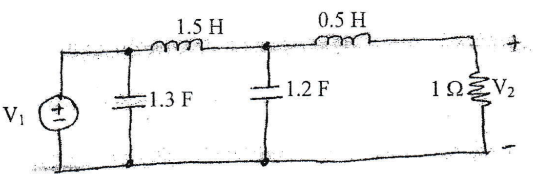
\includegraphics[width=4in]{fd_5}
		\end{enumerate}

	\pagebreak

\section{Approximation Methods}
	\begin{center}(8 Hours/14 Marks)\end{center}
		\subsection{Approximation and its importance in filter design}
			\begin{enumerate}
				\item What is approximation in filter design? \hfill [1] (\texttt{81 Ba})
			\end{enumerate}

		\subsection{Butterworth response, Butterworth pole locations, Butterworth filter design from specifications}
			\begin{enumerate}
				\item What are the characteristics of Butterworth response?\hfill[3] (\bo{\texttt{79 Bh}, 73 Ch})
				\lb What are the characteristics of Butterworth filter?\hfill[2] (\bo{75 Ch})

				\item Derive the expression to calculate the order of a Butterworth low pass filter.
				\enter \hfill[4] (\bo{\texttt{80 Bh, 79 Bh}, 80 Bh, 79 Bh, 78 Bh,75 Bh}, 75 Ash) [5] (\bo{69 Ch})

				\item Derive the transfer function of a normalized 4\textsuperscript{th} Butterworth low pass approximation.\hfill[4] (\bo{81 Bh})
				\lb derive for 5\textsuperscript{th}\hfill[4] (\bo{73 Ch})

				\item Calculate the minm order of Butterworth filter with the following specifications:\hfill[3] (\bo{\texttt{81 Bh}})\\
				\w$_p$/\w$_s$ = 1.5 \hspace{6.7cm}
				$\alpha_{max}$ = 1dB, $\alpha_{min}$ = 25dB

				\item Estimate the order of Butterworth filter, along with pole locations and transfer functions, having following specifications: \\
				a. \w$_p$/\w$_s$ = 1.5 \hspace{5.2cm} $\alpha_{max}$ = 1dB, $\alpha_{min}$ = 20dB\hfill[2+4] (75 Ash)\\
				b. \w$_p$ = 1000rad/s, \w$_s$ = 2000rad/s \hspace{1.5cm}
				$\alpha_{max}$ = 0.5dB, $\alpha_{min}$ = 20dB\hfill[3+3] (\bo{\texttt{80 Bh}, 80 Bh})

				\item Calculate the order of Butterworth filter with the following specifications:\\
				a. \w$_p$ = 2000rad/s, \w$_s$ = 3000rad/s \hspace{3cm}
				$\alpha_{max}$ = 1dB, $\alpha_{min}$ = 12dB \hfill[3] (\bo{\texttt{79 Bh}})\\
				b. \w$_p$ = 2000rad/s, \w$_s$ = 3000rad/s \hspace{3cm}
				$\alpha_{max}$ = 0.5dB, $\alpha_{min}$ = 22dB \hfill[3] (\bo{78 Bh})\\
				c. \w$_p$ = 1000rad/s, \w$_s$ = 2000rad/s \hspace{3cm}
				$\alpha_{max}$ = 1dB, $\alpha_{min}$ = 20dB \hfill[3] (\bo{75 Ch})\\
				d. \w$_p$ = 200rad/s, \w$_s$ = 2000rad/s \hspace{3.2cm}
				$\alpha_{max}$ = 0.1dB, $\alpha_{min}$ = 30dB \hfill[3] (\bo{69 Ch})
			\end{enumerate}
		\subsection{Chebyshev and inverse Chebyshev characteristics, network functions and pole zero locations}
			\begin{enumerate}
				\item What are the characteristics of chebyshev magnitude response?\hfill [3] (81 Ba, \texttt{80 Ba})
				\lb characteristics of chebyshev filter.\hfill[2] (76 Ash)

				\item What are the characteristics of inverse Chebyshev response? \hfill [2] (\bo{\texttt{81 Bh}}, 74 Ash)

				\item Derive the expression to calculate the order of a lowpass Chebyshev filter.
				\enter\hfill[3] \begin{small}(\bo{81 Bh, 74 Ch})\end{small} [4] \begin{small}(\bo{76 Ch}, \texttt{80 Ba})\end{small} [5] \begin{small}(\bo{70 Ch}, 76 Ash, 71 Shr)\end{small} [6] \begin{small}(79 Ba)\end{small}
				\lb  also derive for response.\hfill[7] (\bo{79 Bh})
				\lb and then prove that locus of its pole is an ellipse centered at origin.\hfill[4] (\bo{81 Bh})
				\lb\lb Show that the poles of chebyshev filter lie on an ellipse. Also show the major and minor axes.\hfill[7] (\bo{73 Ch})

				\item Derive the expression to calculate the order of inverse Chebyshev low pass filter. \hfill [3] (\bo{\texttt{81 Bh}})
				\enter \hfill[4] (74 Ash) [5] (\bo{72 Ch, 71 Ch}, \texttt{81 Ba}, 80 Ba, 70 Asa)

				\item Calculate inverse Chebyshev poles and zeros for given specifications: $\boldsymbol{\alpha_{min}}$ = 18dB, $\boldsymbol{\alpha_{max}}$ = 0.25dB, $\boldsymbol{\omega_s}$ = 1400rad/sec and $\boldsymbol{\omega_p}$ = 1000rad/sec. \hfill [5] (\bo{\texttt{81 Bh}})

				\item Determine the  minimum order n of CLPF for following specifications.\\
				$\alpha_p$ = 1dB, $\alpha_s$ = 25dB and (\w\textsubscript{s}/\w\textsubscript{p}) = 1.5, where the symbols have their usual meanings.

				\item Find the minimum order with its transfer function, of CLPF having the specifications:\\
				a. \w$_p$/\w$_s$ = 1.5rad/s \hspace{5.8cm}
				$\alpha_{max}$ = 1dB, $\alpha_{min}$ = 25dB \hfill [3] (\texttt{80 Ba})\\ 
				b. \w$_p$ = 1rad/s, \w$_s$ = 2.33rad/s \hspace{3.7cm}
				$\alpha_{max}$ = 0.5dB, $\alpha_{min}$ = 22dB \hfill[8] (72 Ka)

				\item Estimate the order of CLPF with the following specifications:\\
				a. \w$_p$ = 100Krad/s, \w$_s$ = 140Krad/s \hspace{2.8cm}
				$\alpha_{max}$ = 0.25dB, $\alpha_{min}$ = 18dB\hfill [3] (\texttt{81 Ba})\\
				b. \w$_p$ = 1500rad/s, \w$_s$ = 4500rad/s \hspace{3cm}
				$\alpha_{max}$ = 0.5dB, $\alpha_{min}$ = 20dB \hfill[3] (81 Ba)\\
				c. \w$_p$ = 2000rad/s, \w$_s$ = 2000rad/s \hspace{30.5mm}
				$\alpha_{max}$ = 0.5dB, $\alpha_{min}$ = 22dB \hfill[3] (\bo{79 Bh})\\
				d. \w$_p$ = 2000rad/s, \w$_s$ = 3000rad/s \hspace{3cm}
				$\alpha_{max}$ = 0.5dB, $\alpha_{min}$ = 22dB \hfill[3] (79 Ba)\\
				e. \w$_p$ = 1000rad/s, \w$_s$ = 1500rad/s \hspace{30.5mm}
				$\alpha_{max}$ = 0.25dB, $\alpha_{min}$ = 20dB \hfill[3] (\bo{76 Ch})\\
				f. \w$_p$ = 1000rad/s, \w$_s$ = 2500rad/s \hspace{3.1cm}
				$\alpha_{max}$ = 0.25dB, $\alpha_{min}$ = 40dB \hfill[3] (76 Ash)\\
				g. \w$_p$ = 3200Hz, \w$_s$ = 9800Hz \hspace{3.95cm}
				$\alpha_{max}$ = 0.4dB, $\alpha_{min}$ = 52dB \hfill[3] (\bo{74 Ch})\\
				h. \w$_p$ = 1000rad/s, \w$_s$ = 1400rad/s \hspace{3cm}
				$\alpha_{max}$ = 0.25dB, $\alpha_{min}$ = 18dB \hfill[3] (\bo{71 Ch})\\
				i. \w$_p$ = 1000rad/s, \w$_s$ = 2000rad/s \hspace{3.1cm}
				$\alpha_{max}$ = 0.5dB, $\alpha_{min}$ = 20dB \hfill[3] (71 Shr)\\
				j. \w$_p$ = 1000rad/s, \w$_s$ = 2500rad/s \hspace{3.1cm}
				$\alpha_{max}$ = 0.1dB, $\alpha_{min}$ = 20dB \hfill[3] (\bo{70 Ch})\\
				k. \w$_p$ = 1000rad/s, \w$_s$ = 1800rad/s \hspace{3cm}
				$\alpha_{max}$ = 0.5dB, $\alpha_{min}$ = 18dB \hfill[3] (70 Asa)

				\item Estimate the order of ICLPF with the following specifications:\\
				a. \w$_p$ = 1000rad/s, \w$_s$ = 1800rad/s \hspace{3cm}
				$\alpha_{max}$ = 0.5dB, $\alpha_{min}$ = 25dB \hfill[3] (80 Ba)\\
				b. \w$_p$ = 10000rad/s, \w$_s$ = 20000rad/s \hspace{2.5cm}
				$\alpha_{max}$ = 0.4dB, $\alpha_{min}$ = 16dB \hfill[2] (74 Ash)\\
				c. \w$_p$ = 1000rad/s, \w$_s$ = 1400rad/s \hspace{3cm}
				$\alpha_{max}$ = 0.25dB, $\alpha_{min}$ = 18dB \hfill[2] (\bo{72 Ch})
				\end{enumerate}
				\subsection{Characteristics of Cauer (elliptic) response}
				\begin{enumerate}
				\item What are the characteristics of Elliptic Response?\hfill[3] (73 Shr, 71 Shr)
				\item Compare elliptical response with chebyshev and inverse chebyshev response\hfill[2+2] (73 Shr)
				\lb compare with inverse chebyshev response.\hfill[3] (71 Shr)
			\end{enumerate}
		\subsection{Bessel-Thomson approximation of constant delay}
			\begin{enumerate}
				\item What is constant delay filter?
				\enter[1] \begin{footnotesize}(\bo{80 Bh, 70 Ch}, \texttt{81 Ba, 80 Ba}, 79 Ba, 76 Ash, 74 Ash, 73 Shr, 70 Asa)\end{footnotesize} [2] \begin{footnotesize}(\bo{75 Ch, 69 Ch}, 80 Ba, 75 Ash)\end{footnotesize}

				\item What is significance of constant delay filter?\hfill[1] (\bo{76 Ch}, \texttt{80 Ba}, 76 Ash) [2] (79 Ba)

				\item What are the characteristics of Bessel-Thomson filter?\hfill[2] (\bo{78 Bh})

				\item Derive a transfer function of a second order constant delay filter.
				\enter\hfill[3] (\texttt{80 Ba}, 73 Shr) [4] (\bo{74 Ch}, 76 Ash, 74 Ash)

				\item Find the transfer function of 3\textsuperscript{rd} order Bessel Thomson low pass filter.
				\enter \hfill[3] \begin{footnotesize}(\bo{\texttt{79 Bh}, 75 Ch}, 79 Ba)\end{footnotesize} [4] \begin{footnotesize}(\bo{\texttt{80 Bh}, 80 Bh, 78 Bh, 76 Ch, 69 Ch}, \texttt{81 Ba}, 75 Ash)\end{footnotesize} [5] \begin{footnotesize}(80 Ba)\end{footnotesize}
				\lb for 4th order.\hfill[3] (\bo{71 Ch})

				\item What are the steps involved in designing constant delay filter? Explain with example.\hfill[5] (\bo{70 Ch})
				\lb same question, but with example of 2nd order filter.\hfill[5] (70 Asa)
			\end{enumerate}

		\subsection{Delay Equalization}
			\begin{enumerate}
				\item What is delay and delay equalization? Explain with necessary figures \hfill[2+3] (\bo{79 Bh})
				\lb What is delay equalization?\hfill[1] (\bo{72 Ch}. 72 Ka)

				\item What do you mean by phase and gain equalization.\hfill[2] (\bo{81 Bh})

				\item What is the importance of all pass filters in delay equalization?\hfill[2] (\bo{\texttt{79 Bh}}) [3] (\bo{71 Ch})

				\item Mention the importance of delay equalization.\hfill[3] (74 Ash)

				\item How is delay equalization done? Explain with necessary figures.\hfill[3] (72 Ka) [4] (\bo{72 Ch})
			\end{enumerate}

	\pagebreak
\section{Frequency transformation}
	\begin{center}(2 Hours/4 Marks)\end{center}
	\subsection{Frequency transformation and its importance in filter design}
		\begin{enumerate}
			\item What is frequency transformation (\bo{FT})?
			\enter \hfill [1] (\bo{\texttt{79 Bh}, 81 Ba, 78 Bh, 76 Ch, 75 Ch, 69 Ch}, 80 Ba, 79 Ba, 76 Ash, 74 Ash, 72 Kar) [2] (\bo{74 Ch, 73 Ch})
			
			\item What is the importance of FT? \hfill [1] (\bo{78 Bh, 75 Ch, 70 Ch}, 81 Ba, 76 Ash, 75 Ash, 70 Asa) [2] (\bo{71 Ch})
			
			\item How FT reduces the design steps required to design a filter? \hfill [1] (\bo{\texttt{80 Bh}})
			
			\item What are the application of FT in filter design? \hfill[1] (\texttt{80 Ba}) [2] (\bo{72 Ch})
		\end{enumerate}

	\subsection{Lowpass to highpass transformation}
		\begin{enumerate}
			\item How can you obtain a high pass filter from a given low pass filter? Explain with suitable example.
			\enter \hfill[4] (\bo{72 Ch}, \texttt{80 Ba}, 80 Ba)
			
			\item The following LPF has passband frequency \w\textsubscript{p} of 1 rad/s. Transform it into a highpass filter having passband frequency of 2KHz. \hfill [4] (73 Shr)\\
			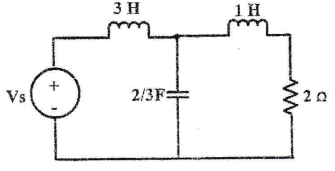
\includegraphics[width=4in]{fd_9}
		\end{enumerate}

	\subsection{Lowpass to bandpass transformation}
		\begin{enumerate}
			\item Describe the frequency transformation from LPF to BPF with a suitable example.
			\enter \hfill [3] (\bo{70 Ch, 69 Ch}) [4] (74 Ash, 70 Asa) [5] (\texttt{81 Ba}, 81 Ba, 71 Shr)
			\lb Derive the expression of RLC for FT from normalized LPF to BPF. \hfill [5] (\bo{79 Bh})
			
			\item Design a Band pass filter having center frequency at 1500 rad/sec and bandwidth 300 rad/sec from a 4\textsuperscript{th} order Butterworth low pass resistively terminated lossless filter. \textit{[\hyperref[sec:tables_81bh]{Refer Table]}}.
			\enter \hfill [4] (\bo{\texttt{81 Bh}})
			\lb  \w \textsubscript{0} = 1 Krad/s, BW = 100 rad/s. \hfill [5] (\bo{78 Bh})
			
			\item Obtain the BPF from LPF given in figure 1 having center frequency 10\textsuperscript{4} rad/s and bandwidth of 9.9 x 10\textsuperscript{4} rad/s. \hfill[4] (\bo{73 Ch})
			
			\item Obtain a bandpass filter having \w\sub{1} = 100 rad/s and \w\sub{2} = 1000 rad/s from following LPF at normalized frequency. \hfill [4] (74 Ash)\\
			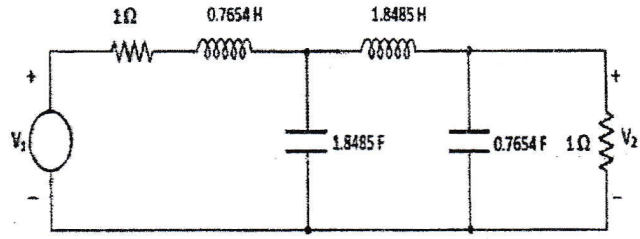
\includegraphics[width=4in]{fd_8}
			
			\item The ckt given below is an LPF having passband frequency of 1 rad/s. Obtain a bandpass filter having \w\sub{0} = 2000 rad/s and B = 400 rad/s. \hfill [3] (\bo{71 Ch})\\
			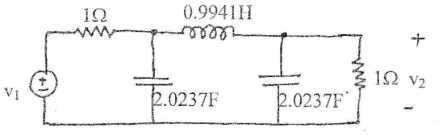
\includegraphics[width=4in]{fd_10}
		\end{enumerate}

	\subsection{Lowpass to bandstop transformation}
		\begin{enumerate}
			\item Explain the frequency transformation technique from a prototype LPF to BSF with necessary derivations.\hfill [3] (72 Kar) [4] (\bo{81 Bh, 74 Ch}, 79 Ba)

			\item Design a bandstop filter having center frequency 2000rad/s and bandwidth 400 rad/s from a 3\textsuperscript{rd} order Butterworth low pass filter. \textit{[\hyperref[sec:tables_81bh]{Refer Table]}}\hfill [4] (\bo{\texttt{80 Bh, 79 Bh}, 76 Ch, 75 Ch})
			\lb from fourth order. \hfill [4] (75 Ash)
			
			\item Following circuit is a low pass filter having $\alpha_p$ = 1dB and \w\sub{p} = 1 rad/s. Obtain a bandpass filter \w\sub{0} = 400 rad/s and bandwidth of 150 rad/s. \hfill [4] (\bo{80 Bh})\\
			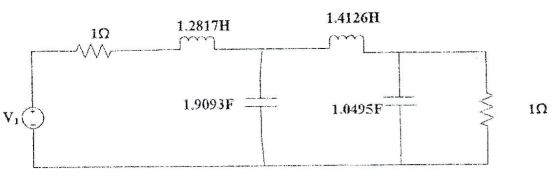
\includegraphics[width=4in]{fd_6}
			
			\item Following filter has cutoff frequency at 1 rad/s. Transform it into a band pass filter having center frequency at 1000 rad/s and bandwidth of 1000 rad/s.\hfill [3] (76 Ash)\\
			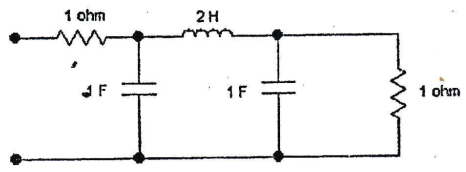
\includegraphics[width=4in]{fd_7}
		\end{enumerate}

	\pagebreak
\section{Properties and Synthesis of Passive Networks}
	\begin{center}(7 Hours/13 Marks)\end{center}
	\subsection{One-port passive circuits}
		\subsubsection{Properties of passive circuits, positive real functions}
			\begin{enumerate}[noitemsep, topsep=0pt]
				\item What are the required properties of a function to be realizable? \hfill [3] (71 Shr)
			\end{enumerate}
			
		\subsubsection{Properties of lossless circuits}
			\begin{enumerate}[noitemsep, topsep=0pt]
				\item Write the properties of lossless one port network. \hfill [2] (\bo{81 Bh}, 76 Ash, 74 Ash) [3] (\bo{78 Bh, 76 Ch})
				
				\item How can you determine whether the given function is a valid lossless function or not? \hfill [3] (81 Ba)
				
				\item Determine whether the following are lossless function or not? State with reason. 
				\enter\hfill [3+3+3] (\bo{78 Bh})\\
				$Z(s) = \dfrac{s^4+9s^2+8}{s^3+4s}2$ \hspace{1cm}
				$Z(s) = \dfrac{s^3+s}{s^4+12s^2+32}$ \hspace{1cm}
				$Z(s) = \dfrac{s^3+4s}{s^4+4s^2+3}$\\
				Realize one of the valid lossless function using Foster Series and Cauer I methods.
			\end{enumerate}

		\subsubsection{Synthesis of LC one-port circuits, Foster and Cauer circuits}
			\begin{enumerate}
				\item What are the properties of LC driving point impedance function? \hfill [3] (\bo{\text{79 Bh}}, \texttt{81 Ba})
				
				\item Which of the function is LC driving point impedance function? \hfill [2+3] (\bo{\texttt{79 Bh}})\\
				$Z(s) = \dfrac{8s^3+10s}{s^4+6s^2+5}$, \hspace{1cm} $Z(s) = \dfrac{s^4+5s^2+4}{s^3+9s}$

				\item Which of the following function is lossless and why? Find the Cauer-I and Foster-I expansion for the corresponding lossless function. \hfill [2+3+3] (\bo{\texttt{81 Bh}})
				\begin{align*}
					Z(S) &= \frac{S^2+10S+24}{S^2+8S+15}\\
					Z(S) &= \frac{S^5+10S^3+24S}{S^4+6S^2+5}
				\end{align*}

				\item Synthesize the given LC function in Foster I and Foster II networks: \hfill [6] (\bo{81 Bh})\\
				$F(s) = \dfrac{s(s^2+2)(s^2+4)}{(s^2+1)(s^2+3)}$
				
				\item Synthesize the given LC impedance in Foster II and Caer I networks: \hfill [3+3] (\bo{79 Bh})\\
				$Z(s) = \dfrac{(s^2+1)(s^2+3)}{s(s^2+2)}$
				
				\item Realize the fllowing function using Cauer I and Foster II method. \hfill [3+3] (74 Ash)\\
				$Z(s) = \dfrac{s(s^2+4)}{(s^2+2)(s^2+6)}$
				
				\item Realize the given function using Cauer-I and Cauer-II method. \hfill [6] (72 Ka)\\
				$Z(s) = \dfrac{4s^4+40s^2+36}{s^3+4s}$
				
				\item Realize the following LC function using Cauer II method. $Z(s) = \dfrac{s(s^2+3)}{(s^2+1)(s^2+4)}$ \hfill [4] (70 Asa)
				
				
				\item Which of the following function is valid LC driving point impedance function? State with reason.
				$Z(s) = \dfrac{8s^3+10s}{s^4+6s^2+5}$,\hspace*{1cm}    $Z(s) = \dfrac{(s^2+4)(s^2+9)}{(s^2+16)(s^2+25)}$ \hfill [3+3] (\texttt{81 Ba})\\
				Find the Cauer second from of valid driving point impedance function.
				
				\item Which of the following functions are the valid LC impedance function? State with reason.\\
				$Z(s) = \dfrac{(s^2+2)(s^2+4)}{s(s^2+1)(s^2+3)}$, \hspace{1cm} $Z(s) = \dfrac{(s^1+1)(s^2+3)}{(s^2)(s^2+4)}$, \hspace{1cm} $Z(s) = \dfrac{(s^2+1)(s^2+3)}{s(s^2+2)(s^2+4)}$\\
				Pick one valid LC impedance function and realize it in Foster I and Cauer II form. 
				\enter\hfill [3+3+3] (81 Ba)
				
				\item Which of the following is valid lossless function? State with reason. \\
				$Z(s) = \dfrac{(s^2+4)(s^2+5)}{(s^2+s^2)(s^2+10)}$, \hspace{1cm} $Z(s)= \dfrac{s^4+4s^2+3}{s(s^2+2)}$, \hspace{1cm} $Z(s) = \dfrac{s^6+4s^4+8s^2}{s^3+3s}$\\
				Pick one of the valid LC lossless functions and synthesize it using
				\lb Foster II and Cauer II methods. \hfill [3+3+3] (\bo{\texttt{80 Bh}})
				\lb Foster series nd cauer I methods. \hfill [2+3+3] (\bo{80 Bh})
				
				\item Which of the following functions are LC driving point impedance function and why?\\
				$Z_1 (s)=\dfrac{(s^2+1)(s^2+5)}{(s^2+2)(s^2+10)}$ \hspace{2cm}
				$Z_2 (s)=\dfrac{5s(s^2+5)}{(s^2+1)(s^2+2)}$\\[2pt]
				$Z_3 (s)=\dfrac{2(s^2+1)(s^2+9)}{s(s^2+4)}$ \hspace{2cm}
				$Z_4 (s)=\dfrac{4(s+2)(s+5)}{(s+1)(s+4)}$\\
				Pick one of the valid LC driving point impedance and synthesize it in Foster-I and Cauer-I form.
				\enter\hfill [2+3+3] (79 Ba)
				
				\item Which of the following function is LC one port driving point impedance function? Explain with suitable reason. \hfill [2+3+3] (\bo{76 Ch})\\
				$Z(s) = \dfrac{(s^2+1)(s^2+9)}{s(s^2+4}$, \hspace{2cm}
				$Z(s) = \dfrac{s(s^2+4)(s^2+5)}{(s^2+3)(s^2+6)}$\\
				Realize a valid lossless one part function using Foster II and Cauer II methods.
				
				\item Which of the following are valid LC function? State with reason. Realize one LC function using Cauer-I and Cauer-II method. \hfill [2+3+3] (76 Ash)\\
				$Z(s) = \dfrac{(s^2+1)(s^2+3)}{s(s^2+2)}$ \hspace{2cm}
				$Z(s) = \dfrac{s(s^2+2)}{(s^2+3)(s^2+4)}$
				
				\item Determine whether the following functions are lossless function or not? State with reason. \\
				$Z(s) = 2\dfrac{s^4+9s^2+8}{s^3+4s}$ \hspace{2cm}
				$Z(s) = \dfrac{s^3+s}{s^4+12s^2+32}$ \hspace{2cm}
				$Z(s) = \dfrac{s^4+4s}{s^4+4s+3}$
				Realize one of the valid lossless function using Foster Series method and Cauer II method.
				\enter\hfill [3+3+3] (\bo{75 Ch})
				
				\item Which of the following is LC lossless functions and why? Pick one of the valid LC lossless functions and realize it using Foster-I and Cauer-I form. \hfill [3+3] (75 Ash)\\
				$Z_1(s) = \dfrac{s(s^2+4)(s^2+6)}{(s^2+3)(s^2+9)}$ \hspace{2cm}
				$Z_2(s) = \dfrac{(s^2+3)(s^2+6)}{s(s^2+4)(s^2+9)}$ \\
				$Z_3(s) = \dfrac{(s^2+4)(s^2+6)}{s(s^2+3)(s^2+9)}$ \hspace{2cm}
				$Z_4(s) = \dfrac{(s^2+3)(s^2+6)}{(s^2+4)(s^2+9)}$
				
				\item Which of the following functions are LC driving point impedance function and why?\\
				$Z(s) = \dfrac{s^4+10s^2+9}{s^4+4s}$ \hspace{2cm}
				$Z(s) = \dfrac{s^3+4s}{s^4+5s^2+6}$\hfill [2+3+3] (73 Shr)\\
				Also find the Foster parallel and cauer I form of the valid LC driving point impedance function.
				
				\item Which of the following is LC lossless function and why? Pick one of the valid LC lossless functions and synthesize it using Foster and Cauer methods. \hfill [2+3+3] (\bo{72 Ch})\\
				$Z_1(s)=\dfrac{s(s^2+4)(s^2+9}{(s^2+2)(s^2+10}$ \hspace{2cm}
				$Z_2(s)=\dfrac{(s^2+2)(s^2+10)}{s(s^2+5)}$ \hspace{2cm}
				$Z_3(s)=\dfrac{s^2+25}{s(s^2+5)(s^2+50)}$
				
				\item Which of the following functions are LC driving point impedance function and why? Also find the Foster series and Caucer II Realization of the valid LC driving point impedance function.\\
				$Z(s) = 2\dfrac{(s^2+4)(s^2+16}{(s^2+1)(s^2+9}$ \hspace{2cm}
				$Z(s) = 4\dfrac{(s+2)(s+5)}{(s+1)(s+4)}$ \hfill [2+3+3] (\bo{71 Ch})
				
				\item Which of the following functions are LC driving point impedance function and why? Pick one of the valid LC driving point impedance and synthesize it in Foster-I and Caver-I form:\\
				$Z_1(s) = \dfrac{(s^2+1)(s^2+5}{(s^2+2)(s^2+10)}$ \hspace{2cm}
				$Z_2(s) = \dfrac{5s(s^4+4)}{(s^2+1)(s^2+3)}$ \hfill [2+3+3] (\bo{70 Ch})\\
				$Z_3(s) = \dfrac{2(s^2+1)(s^2+9)}{s(s^2+4)}$ \hspace{2cm}
				$Z_4(s) = 4\dfrac{(s+2)(s+5)}{(s+1)(s+4)}$
				
				\item Which of the following functions are LC driving point impedance and why? \hfill [4+3] (\bo{69 Ch})\\
				$Z(s) = \dfrac{s(s^2+4)}{(s^2+9)(s^2+16)}$, \hspace{2cm}
				$Z(s) = \dfrac{s(s^2+1)(s^2+9)}{(s^2+4)(s^2+16)}$ \\
				$Z(s) = \dfrac{s(s^2+4)}{2(s^2+1)(s^2+9)}$, \hspace{2cm}
				$Z(s) = \dfrac{2(s+1)(s+3)}{(s+2)(s+4)}$\\
				Also find the Cauer II realization of the valid LC driving point impedance function.
				
				\item Synthesize a two port LC ladder to satisfy the following open circuit impedance parameters: $z_{21}(s) = \dfrac{k(s^2+9}{s(s^2+4}$; $z_{22}(s) = \dfrac{(s^2+1)}{s(s^2+4)}$ \hfill [7] (72 Ka)
			\end{enumerate}

		\subsubsection{Properties and synthesis of RC one-port circuits}
			\begin{enumerate}
				\item What are the properties of RC impedance function?\hfill [2] (\bo{74 Ch}) [3] (\bo{75 Ch}, \texttt{80 Ba}, 80 Ba)
				\lb Explain with example. \hfill [4] (70 Asa)
				
				\item Synthesize the given RC impedance in Foster and Cauer form.\hfill[3+3] (\texttt{80 Ba})\\
				$Z(s) = \dfrac{3(s+2)(s+4)}{s(s+3)}$
				
				\item Which of the following are valid RC driving point impedance function and why? \hfill [5] (80 Ba)\\
				$Z(s) = \dfrac{\text{(s+3)(s+6)}}{\text{(s+1)(s+5)}}$, \hspace{1cm} $Z(s) = \dfrac{\text{2(s+1)(s+3)}}{\text{(s+2)(s+4)}}$\\
				Find Foster form of valid RC driing point impedance function.
				
				\item Which of the following is valid RC impedance function? State with reason. Pick a valid RC impedance function and realize it using foster I and cauer I method. \hfill [2+3+3] (\bo{74 Ch})\\
				$z(s) = \dfrac{s(s^2+2)}{(s^2+1)}$ \hspace{2.8cm}
				$z(s) = \dfrac{(s+1)(s+5)}{(s+3)(s+7)}$ \\
				$z(s) = \dfrac{(s+4)(s+7)}{(s+1)(s+5)}$ \hspace{2cm}
				$z(s) = \dfrac{(s+1)(s+3)}{(s+4)(s+5)}$ 
				
				\item Which of the following functions are lossless impedance function? State with reason. 
				\enter\hfill [2+3+3] (\bo{73 Ch})\\
				$\dfrac{(s^2+1)(s^2+9)}{(s^2+4)(s^2+16)}$ \hspace{1cm}
				$\dfrac{s(s^2+4)}{(s^2+1)(s^2+3)}$ \hspace{1cm}
				$\dfrac{2(s^2+1)(s^2+9)}{s(s^2+4)}$ \hspace{1cm}
				$\dfrac{s^5+4s^3+5s}{s^4+5s^2+6}$\\
				Synthesize one of the valid lossless impedance function using Foster I and Cauer I forms.	
				
				\item Which of the following function is valid RC admittance function? State with reason. Realize one of the RC admittance function in Foster II and RC ladder form. \hfill [2+3+3] (71 Shr)\\
				$Y(s) = \dfrac{(s+1)(s+3)}{(s+2)(s+4)}$, \hspace{2cm}
				$Y(s) = \dfrac{(s^2+1)(s^2+3)}{(s^2+2)(s^2+4)}$\\
				$Y(s) = \dfrac{(s+2)(s+4)}{(s+1)(s+3)}$, \hspace{2cm}
				$Y(s) = \dfrac{(s+1)(s+3)}{s(s+2)(s+4)}$
			\end{enumerate}

	\subsection{Two-port Passive Circuits}
		\begin{enumerate}[noitemsep, topsep=0pt]
			\item What do you mean by 2-port network? \hfill [1] (\bo{\texttt{81 Bh}}) 
		\end{enumerate}

		\subsubsection{Properties of passive two-port circuits, residue condition, transmission zeros}
			\begin{enumerate}[noitemsep, topsep=0pt]
				\item Explain the properties of lossless two port function. \hfill [3+3] (71 Shr)

				\item What is called poles and transmission poles. \hfill [1] (\bo{80 Bh})

				\item Define transmission zeros in two port network.
				\enter\hfill [1] \begin{footnotesize}(\bo{\texttt{80 Bh}, 80 Bh, 76 Ch, 75 Ch, 74 Ch, 73 Ch, 72 Ch, 71 Ch, 70 Ch}, \texttt{81 Ba}, 80 Ba, 79 Ba, 75 Ash, 70 Asa)\end{footnotesize} [2] \begin{footnotesize}(\bo{\texttt{79 Bh}})\end{footnotesize}
				
				\item How can zeros of transmission be realized in ckts?
				\lb Explain with suitable diagrams. \hfill [4] (\bo{\texttt{79 Bh}, 76 Ch}) [5] (\bo{75 Ch}, \texttt{81 Ba})
				\lb Explain with examples. \hfill [3] (79 Ba) [4] (\bo{74 Ch, 73 Ch, 72 Ch, 71 Ch}, 70 Asa)
				
				\item What are the different ways of producing zeros in a network realization? \hfill [3] (\bo{80 Bh})
				\lb Explain with examples. \hfill [5] (80 Ba)

				\item Explain the conversion of Z parameters in terms of Y parameters with necessary derivation for a two port passive network. \hfill [5] (\bo{81 Bh})	
				
				\item Explain the series connection of two 2 port networks with figure and derivation. \hfill [4] (\bo{\texttt{81 Bh}})
			\end{enumerate}

		\subsubsection{Synthesis of two-port LC and RC ladder circuits based on zero-shifting by partial pole removal}
			\begin{enumerate}
				\item What is zero shifting? \hfill [2] (81 Ba)
				
				\item How is zero shifting useful for two port networks synthesis? Explain with examples. \hfill [4] (81 Ba)
				
				\item What is zero shifting by partial removal of pole? \hfill [1] (73 Shr)
				\lb Explain w/ suitable example.\hfill [3] (\bo{\texttt{80 Bh}}, 75 Ash) [4] (\bo{71 Ch, 69 Ch}) [5] (\texttt{80 Ba})
				\lb Explain its signficance with example. \hfill [5] (\bo{78 Bh})
				
				\item Explain importance of zero shifting in two port network synthesis. \hfill [2] (\bo{69 Ch})

				\item What do you mean by partial removal and complete of pole in the synthesis of 2-port lossless ladder network? Explain w/ examples. \hfill [6] (\bo{79 Bh})
				\lb How can two-port passive circuits be synthesized using zero-shifting by partial pole removal? Explain. \hfill [4] (73 Shr)
			\end{enumerate}

	\pagebreak
\section{Design of Resistivety-Terminated Lossless Fitter}
	\begin{center}(4 Hours/7 Marks)\end{center}
	\subsection{Properties of resistively-terminated lossless ladder circuits, transmission and reflection coefficients}
		\begin{enumerate}
			\item What is reflection coefficient? \hfill [1] (\bo{\texttt{79 Bh},80 Bh, 70 Ch}, 73 Shr, 70 Asa) [1.5] (74 Ash)
		
			\item What is transmission coefficient? \hfill [1] (\bo{71 Ch, 69 Ch}, \texttt{80 Ba}, 73 Shr) [1.5] (74 Ash)
		
			\item What information do you get from transmission coefficient? \hfill [1] (\bo{75 Ch, 71 Ch, 69 Ch}, \texttt{80 Ba})

			\item Describe the significance of reflection coefficient.\hfill [2] (\bo{\texttt{80 Bh}}, 80 Ba)
		
			\item What information do you get from reflection coefficient? \hfill [1] (\bo{75 Ch, 74 Ch})
		
			\item What information do you get when the value of reflection coefficient is zero?\hfill [1] (\bo{78 Bh}, \texttt{81 Ba})
			
			\item What do you understand when the transmission coefficient has unity value? \hfill [1] (72 Ka)
		
			\item Derive the expression for reflection coefficient for a resistively terminated LC ladder network.
			\enter\hfill [5] (\bo{71 Ch}, \texttt{80 Ba})
		
			\item What is transmission coefficient? What information do we get from it?\hfill[2] (80 Ba)
		
			\item Realize the 3\super{rd} order Butterworth high pass filter using transfer function of LPF as $T(S)= \dfrac{1}{(S+1)(S^2+S+1)}$ in the form of doubly terminated LC ladder with R\sub{1} = R\sub{2}=1\W. \hfill [5] (\bo{\texttt{81 Bh}})
		
			\item Design a third order Butterworth low pass using a doubly terminated lossless ladder such that the transmission coefficient is T(s) = $\dfrac{1}{(s+1)(s^2+s+1)}$; with R1 = 1\W and R2 = 4\W. \hfill [5] (79 Ba)
		
			\item Design low pass filter using a doubly terminated lossless ladder such that the transmission coefficient is T(s) = $\dfrac{1}{(s+1)(s^2+s+1)}$; Having R1 = 1\W, and R2 = 4\W. \hspace{2.1cm} [7] (76 Ash)
		
			\item Realize the 3\super{rd} order Butterworth high pass filter in the form of doubly terminated ladder with R\sub{1} = R\sub{2}=1\W. \hfill [6] (\bo{80 Bh})
		
			\item Design a third order Butterworth low pass filter using Resistively terminated lossless ladder with equal termination of 1\W. \textit{[\hyperref[sec:tables_81ba]{Refer Table]}} \hfill [5] (\bo{74 Ch, 69 Ch}, 70 Asa) [6] (\bo{70 Ch}, 72 Ka)
		
			\item Design a third order Butterworth low pass filter using Resistively terminated lossless ladder with equal termination of 1\W. \textit{[\hyperref[sec:tables_81ba]{Refer Table]}} \hfill [5] (\bo{78 Bh}) [6] (\bo{81 Bh}, \texttt{81 Ba})
		
			\item Realize a third order Butterworth low pass filter using resistively terminated lossless ladder with R\sub{1} = 1\W and R\sub{2} = 4\W. \textit{[\hyperref[sec:tables_81bh]{Refer Table]}} \hfill [5] (\bo{\texttt{79 Bh}})
		
			\item Derive the 3\super{rd} order Butterworth low pass filter resistively-terminated lossless network with unequal termination of R\sub{1} = 1\W and R\sub{2} = 4\W. \hfill [5] (\bo{\texttt{80 Bh}}) [6] (\bo{79 Bh}) [7] (\bo{72 Ch}, 75 Ash)

			\item Design a third order Butterworth low pass filter using a doubly terminated lossless ladder having R\sub{1} = 1\W and R\sub{2} = 4\W. \textit{[\hyperref[sec:tables_81bh]{Refer Table]}} \hfill [6] (\bo{76 Ch})
		
			\item Design a second order Butterworth low pass filter using resistively terminated terminated lossless ladder with equal termination of 1\W. T(s) = $\dfrac{1}{s^2+\sqrt{2}s+1}$ 
		\enter\hfill [5] (\bo{75 Ch})
	\end{enumerate}

	\subsection{Synthesis of LC ladder circuits to realize all-pole lowpass functions}
		\begin{enumerate}
			\item (assumed) What is GIC? How can it be used to avoid shunt inductors in LC ladder circuit?
			\enter\hfill [5] (81 Bh)

			\item What is GIC? How Antonious' GIC can be used to simulate grounded inductor? Explain with necessary figures and derivations. \hfill [6] (71 Shr)

			\item Realize the following transfer function using LC Ladder with equal termination of R\sub{1} = R\sub{2} = 1\W.\\
			$T(s) = \dfrac{1}{s^2+\sqrt{2}s+1}$ \hfill [5] (80 Ba)
		\end{enumerate}
		
	\subsection{Synthesis of LC ladder circuits to realize functions with finite transmission zeros}
		\begin{enumerate}[noitemsep, topsep=0pt]
			\item How resistively terminated ladder network can be realized with finite transmission zeroes? Explain.
			\enter\hfill [4] (73 Shr)
			
			\item Design a 3\super{rd} order Butterworth HPF in doubly-terminated LC ladder network. \hfill [5] (\bo{81 Bh})
			
			\item Synthesize T(s) = $\dfrac{1}{s^3+2s^2+2s+1}$ in LC ladder circuit terminated with R\sub{1} = R\sub{2} = 1\W.
			\enter\hfill [5] (74 Ash)
			
			\item Realize the third order Butterworth lowpass transfer function T(s) = $\dfrac{1}{s^3+2s^2+2s+1}$ in the form of resistively terminated LC ladder with R\sub{1} = 1\W and R2 = 2\W. \hfill [6] (\bo{73 Ch})
		\end{enumerate}

	\pagebreak
\section{Active Filter}
	\begin{center}(7 Hours/12 Marks)\end{center}
	\subsection{Fundamentals of Active Filter Circuits}
		\subsubsection{Active filter and passive filter}
		\begin{enumerate}
			\item What is active filter? \hfill [1] (\bo{78 Bh})

			\item Differentiate active and passive filter.\hfill [2] (\bo{\texttt{80 Bh}}) [4] (76 Ash)
			
			\item What are the advantages of active filters over passive filters? \hfill [2] (81 Ba) [3] (\bo{76 Ch})
		\end{enumerate}
		
		\subsubsection{Ideal and real operational amplifiers, gain-bandwidth product}
		\subsubsection{Active building blocks: amplifiers, summers, intregrators}
		\subsubsection{First order passive sections and active sections using inverting and non-inverting op-amp configuration}
			\begin{enumerate}
				\item Realize a system using non-inverting op-amp configuration with
				\lb zero at -5 and pole at -3 and having high frequency gain of 2.\hfill[5] (\bo{\texttt{81 Bh}})
				\lb zero at s = -4, pole at s = -8 and high frequency gain of 2. \hfill [5] (\bo{79 Bh})
				\lb zero at 1000, pole at 100 and dc gain of 5. \hfill [3] (\bo{76 Ch})
				\lb zero at -1000 pole at -100 with DC gain of 10. \hfill [5] (80 Ba)

				\item Realize the following transfer function using non-inverting op-amp configuration.
				\lb T(s) = $\dfrac{4(s+2)}{s+1}$ \hfill [3] (\bo{\texttt{80 Bh}})
				\lb T(s) = $\dfrac{4(s+200)}{s+100}$ \hfill [4] (\bo{80 Bh})
				\lb T(s) = $\dfrac{s+8}{s+2}$ \hfill [3] (76 Ash) [4] (\texttt{81 Ba})
				\lb T(s) = $\dfrac{s+8}{s+2}$ \hfill [4] (\bo{78 Bh})

				\item Realize the following transfer function by cascading two first order sections using inverting op-amp configuration.\\
				T(s) = $\dfrac{12}{s^2+8s+12}$ \hfill [6] (\bo{79 Bh})
			\end{enumerate}

	\subsection{Second order active sections (biquads)}
		\begin{enumerate}[noitemsep, topsep=0pt]
			\item What is quality factor and center frequency of LP biquad filter? Explain with diagram.
			\enter\hfill [3] (\bo{\texttt{79 Bh}})
		\end{enumerate}

		\subsubsection{Tow-Thomas biquad circuit, design of active filter using TowThomas biquad}
			\begin{enumerate}
				\item Realize a bilinear transfer function wiht a zero at 800, a pole at 400 and dc gain of 4 using non-inverting op-amp configuration. \hfill [5] (81 Ba)

				\item Draw the circuit diagram of Tow-Thomas Biquad circuit and derive its transfer function. Design a low pass filter using Tow Thomas Biquad circuit with poles at -450 $\pm$ j 893.03 and dc gain of 1.5. The final circuit should contain practically realizable values.\hfill [8] (\bo{\texttt{80 Bh}, 80 Bh, 74 Ch})

				\item Draw the circuit diagram of Tow Thomas LPF pass filter and derive its transfer function. Realize following LPF using Tow Thomas biquad circuit. \hfill [4+4] (73 Shr)\\
				T(s) = $\dfrac{-2000}{s^2+500s+1000000}$
				\lb Realize the following LPF transfer function using Tow-Thomas biquad circuit.\\
				T(s) = $\dfrac{-2000}{s^2+500s+1000000}$ \hfill [5] (\bo{\texttt{79 Bh}})

				\item Derive the transfer function of Tow-Thomas LP biquad filter and design a lowpass filter having poles at -400 $\pm$ j 3979.95 and dc gain of 4 with practically realizable values. \hfill [4+4] (80 Ba)
				\lb dc gain of 1.5, capcacitor value 0.001$\mu$F. \hfill [4+4] (76 Ash)

				\item Derive the transfer function of Tow-Thomas low pass biquad. Design a lowpass filter having poles at -24000 $\pm$ j 32000 and dc gain of 2, with practically suitable elements. \hfill [4+4] (\bo{78 Bh})

				\item Draw the circuit diagram of Tow-Thomas low pass biquad ckt and derive its transfer function. Design a low pass filter using Tow Thomas biquad ckt with poles at 577 $\pm$ j 816.8 and DC gain of 2. Use capacitor of value 0.01$\mu$F in your design. \hfill [4+4] (79 Ba)

				\item Design a second order low pass filter with poles at -10000 $\pm$ j 17320.51 and DC gain of 2.5 using Tow Thomas Biquad Circuit. Your final circuit should have capacitors of value 0.001$\mu$F.
				\enter\hfill [6] (\texttt{80 Ba})
			\end{enumerate}

		\subsubsection{Sallen-Key biquad circuit and Multiple-feedback biquad (MFB) circuit}
			\begin{enumerate}
				\item Draw the circuit diagram of Sallen-Key LP biquad ckt and derive the transfer function.
				\enter\hfill  [4] (81 Ba) [5] (\bo{\texttt{81 Bh}})

				\item Draw the circuit diagram of Sallen-Key LP biquad ckt and derive the transfer function. How can you obtain highpass filter from lowpass one? Design the second order l owpass Butterworth filter having half power frequency of 12KHz using Sallen-Key biquad circuit. \hfill [4+2+4] (74 Ash)\\
				T(s) = $\dfrac{1}{s^2+\sqrt{2}s+1}$

				\item Why gain enhancement is needed in Sallen-Key biquad? Explain the gain enhancement in Sallen Key LP biquad. \hfill [2+4] (\bo{81 Bh})

				\item How can gain enhancement be performed in Sallen-Key circuit? Explain with necessary diagram.
				\enter\hfill [5] (73 Shr)
				
				\item Design a 4\super{th} order Butterworth LPF using cascaded two Sallen-Key biquads having half power frequency of 1 kHz and largest capacitor of 0.1 $\mu$F in your final circuit. \hfill [8] (\bo{79 Bh})
				
				\item Design a MFB LP biquad for the transfer function as $T(s) = \dfrac{5}{s^2+1.2s+1}$ \hfill [4] (\bo{\texttt{81 Bh}})

				\item Derive the transfer function of low pass sallen-key biquad filter \textit{[\hyperref[sec:tables_81ba]{Refer Table]}}. The half power frequency should be 10KHz. Make the largest capacitance 0.01$\mu$F and overall gain be 1.
				\enter \hfill [4+4] (\texttt{81 Ba})

				\item Derive the transfer function of Sallen-Key LPF. Uisng Sallen and Key ckt, design an LPF having \w$_0$ of 1000 rad/s, quality factor of 0.866 and gain of 2. \hfill [4+4] (\bo{73 Ch})

				\item Derive transfer function of Sallen-Key LPF. Design ckt for transfer function T(s) = $\dfrac{1}{s^2+0.76s+1}$ using Sallen-Key LPF. In your final design the values of capacitors must be 0.01$\mu$F and feedback resistors should be equal. \hfill [4+4] (\bo{76 Ch, 75 Ch})

				\item Derive transfer function of Sallen-Key LPF. Design a second order Butterworth LPF using Sallen-Key biquad. In your final design the values of capacitors must be 0.01 $\mu$F and feedback resistors should be equal.. \hfill [4+4] (\bo{75 Ash})

				\item Realize the normalized transfer function of $\dfrac{1}{s^2+s+1}$ using Sallen-Key biquad circuit. In your final design, the half power frequency should be 1.8kHz and all capacitances of 10nF. \hfill [4] (81 Ba)

				\item How is excess gain compensated in Sallen-Key circuit? Explain. \hfill [5] (\bo{74 Ch})
				\lb explain with necessary derivations and diagrams.\hfill [5] (\texttt{80 Ba})

				\item Design a 4\super{th} order Butterworth LPF using cascade two MFB biquads with dc gain equal to unity and half power frequency at 1000rad/s. Make the largest capacitance 0.1 $\mu$F in your final circuit.
				\enter\hfill [8] (\bo{81 Bh})
			\end{enumerate}

		\subsubsection{Cain reduction and gain enhancement}
		\subsubsection{RC-CR transformation}

\pagebreak

\section{Sensitivity}
\begin{center}(3 Hours/5 Marks)\end{center}
\subsection{Sensitivity and importance of sensitivity analysis}
\begin{enumerate}
    \item What is sensitivity? \hfill [1] (81 Ba)
\item What is sensitivity analysis in filter design? \hfill [1] (81 Bh)
\item What is the importance of sensitivity analysis in filter design? \hfill[2] (80 Ba)
\item What information do you get when the sensitivity of y with respect to x is 0.1?\hfill [1] (80 Bh)
\end{enumerate}
\subsection{Definition of single parameter sensitivity}
    \begin{enumerate}[noitemsep, topsep=0pt]
        \item Explain the single parameter and multi-parameter sensitivity. \hfill [2] (81 Ba)
    \end{enumerate}

\subsection{Centre frequency and Q-factor sensitivity}
\begin{enumerate}
\item Perform sensitivity analysis for center frequency $\omega_0$ of Tow Thomas low pass filter with respect to all the resistors and capacitors present in the circuit.\hfill[3] (80 Bh)
\end{enumerate}
\subsection{Sensitivity properties of biquads}
\begin{enumerate}
    \item Perform the sensitivity analysis of coo of Sallen-Key lowpass biquad filter. \hfill [4] (81 Ba)

\item Perform the sensitivity analysis of quality factor (Q) in Tow Thomas low pass biquad.
\enter\hfill [5] (81 Bh)
\item Explain the importance of sensitivity analysis in the design of filter. \hfill[2] (81 Ba)
\item Perform the sensitivity analysis of \W\textsubscript{0} of sallen-key lowpass biquad filter. \hfill [5] (81 Ba)
\enter \hfill [4] (80 Ba)
\end{enumerate}
\subsection{Sensitivity of passive circuits}

\pagebreak
\section{Design of High-Order Active Filters}
\begin{center}(6 Hours/11 Marks)\end{center}
\subsection{Cascade of biquads}
\subsubsection{Sequencing of filter blocks, center frequency, Q-factor and gain}
\subsection{Active simulation of passive filters}
\subsubsection{Ladder design with simulated inductors}
	\begin{enumerate}[noitemsep, topsep=0pt]
		\item What is a generalized impedance converter (GIC)? \hfill [1] (81 Ba)
		
		\item How can you simulate the grounded inductor using GIC? \hfill [3] (81 Ba)
		
		\item From the LC ladder given in figure below, design a highpass filter with a half power frequency of 5 kHz and the largest capacitance of 10nF using inductor simulation. \hfill [5] (81 Ba)\\
		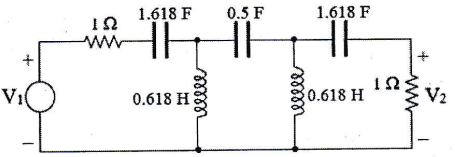
\includegraphics[width=4in]{fd_11}
	\end{enumerate}
\subsubsection{Ladder design with frequency dependent negative resistors (FDNR)}
\begin{enumerate}
\item What is FDNR? How can you use FDNR to avoid the inductor in filter design?\hfill[4] (80 Bh)
\item What is FDNR? How can it be realized?\hfill [1+3] (80 Ba)
\item What is Bruton Transformation? Design the 4\textsuperscript{th} order Butterworth low pass filter with half power frequency 2,000 rad/sec and practically realizable elements using FDNR. \textit{[\hyperref[sec:tables_81bh]{Refer Table]}}.
\enter\hfill [2+4] (81 Bh)
\item Design third order Butterworth low pass filter having half power frequeuncy 4000rad/s using FDNR. \textit{[\hyperref[sec:tables_81bh]{Refer Table]}}.\hfill [6] (80 Bh)
\item Realize the following passive filter using FDNR, having \w\sub{0} = 25000rad/s and practical element values in your final circuit.\hfill[5] (80 Ba)\\
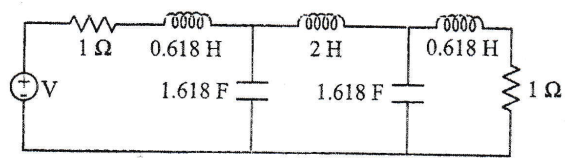
\includegraphics[width=0.5\textwidth]{fd_4}
\end{enumerate}
\subsubsection{Leapfrog simulation of ladders}
\begin{enumerate}
\item Design the 4\textsuperscript{th} order Butterworth LPF in doubly-terminated network using Leapfrog simulation. The necessary information is listed in the given table below:\hspace*{20mm} [8] (81 Ba)\\
\begin{tabular}{|c|c|c|c|c|c|c|}
\hline
Order(n)=4 and LPF & R\(_1$=1 & L$_1$=0.7654 & C$_2$=1.848 & L$_3$=1.848 & C$_4$ = 0.7654 & R$_2$=1\\ \hline
\end{tabular}

\end{enumerate}

\pagebreak
\section{Switched-Capacitor Filters}
\begin{center}(4 Hours/7 Marks)\end{center}
\subsection{The MOS switch and switched capacitor}
\begin{enumerate}
	\item What is the importance of switched capacitor filters? \hfill [2] (81 Ba)

\item Why do we need switched capacitor to simulate resistor in MOS technology?\hfill[2] (80 Ba)
\end{enumerate}
\subsection{Simulation of resistor by switched capacitor}
\begin{enumerate}
\item What is Switch capacitor filter? Design a switched capacitor filter to realize the transfer function.\hfill [6] (81 Ba)\\
$T(s) = \dfrac{(s+200)(s+800}{(s+400)^2}$
\item Why are resistors are replaced by switched capacitors in modern IC technology?\hfill[1] (81 Bh)
\enter\hfill [2] (80 Bh)
\item How can you simulate a resistor using switched capacitor? Explain w/ necessary derivations.
\textcolor{white}{1} \hfill[4] (80 Ba)

\end{enumerate}
\subsection{Switched-capacitor circuits for analog operations: addition, subtraction, multiplication and integration}
\begin{enumerate}
\item Design a switched capacitor filter to realize the magnitude response given by the plot below:
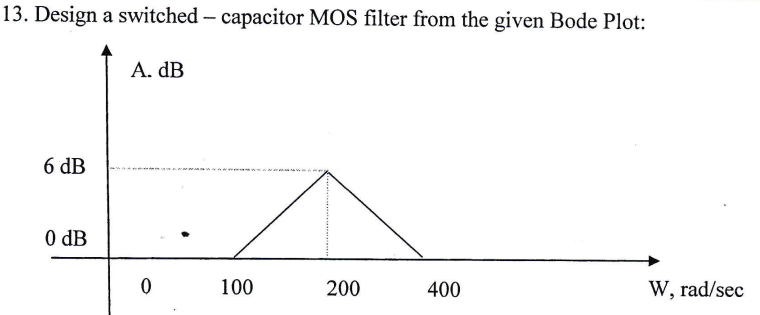
\includegraphics[width=0.5\textwidth]{fd_1} \hfill [6] (81 Bh)

	\item What is the importance of switched capacitor filters? Design a switched capacitor filter to realize the magnitude response specified by the following Bode Plot. \hfill [5] (81 Ba)\\
	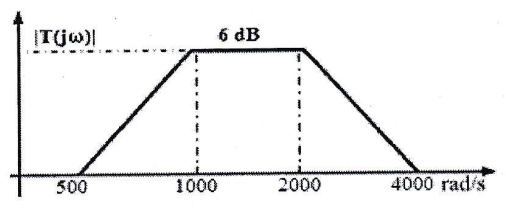
\includegraphics[width=4in]{fd_12}

\item How summer, inverting integrator and non-inverting integrator can be realized using switched capacitor? Explain with necessary diagrams and expressions.\hfill [4] (80 Bh)
\end{enumerate}
\subsection{First-order and second-order switched-capacitor circuits}

\pagebreak
\section{Tables}
\label{sec:tables_81bh}
\subsubsection{81 Bh/80 Bh}
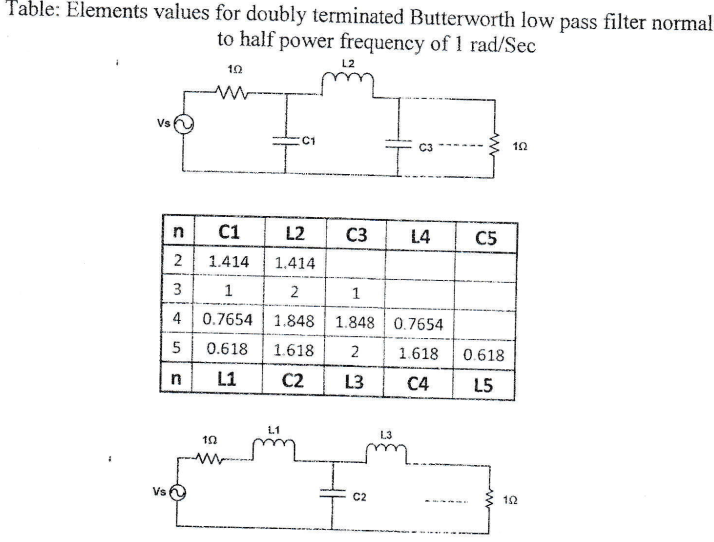
\includegraphics[width=4in]{fd_2}
\label{sec:tables_81ba}
\subsubsection{81 Ba}
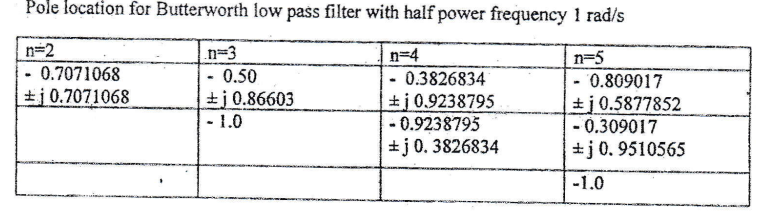
\includegraphics[width=4in]{fd_3}
\label{sec:tables_80bh}
\end{document}
